\section{Artifact Identity and Reproducibility}
\label{app:artifacts}

The experimental record includes exact source/configuration snapshots, fixed
rosters and input hashes, selection/plan publication before evaluation, per-stage
logs, timestamped status events, bootstrap draws and complete report/data
inventories. Output directories are exclusive: no implicit overwrite or resume
is used. Numerical failures stop execution; they do not authorize replacement
roots. Completed and failed/inconclusive scientific outcomes are different
notions. An anonymous release must be prepared before any actual submission;
this working PDF intentionally omits identifying project and sandbox links.

\begin{table}[h]
\caption{Released artifact identities. These upstream identities identify the
audited checkpoints, not an architecture-wide comparison. SHA256 values are
included in the accompanying authenticated evidence ledger.}
\centering\small
\begingroup
\setlength{\tabcolsep}{3pt}
\begin{tabular}{lll}
\toprule
Component & Upstream source/release & Pinned revision \\
\midrule
LeWM source & \texttt{lucas-maes/le-wm} & \texttt{8edfeb336732b5f3ce7b8b210d0ba370a09e2cac} \\
LeWM weights & \texttt{quentinll/lewm-pusht} & \texttt{22b330c28c27ead4bfd1888615af1340e3fe9052} \\
Point implementation/simulator & \texttt{fafraob/point-lewm} & \texttt{1b5a90ebf63e8ef165b1dfe100b81b12f4fa1424} \\
RGB DINO release & \texttt{fafraob/point-cloud-pusht} & \texttt{664278a4c0b4c5f607d0993744986b2d10b4168e} \\
DINOv2 source & \texttt{facebookresearch/dinov2} & \texttt{85a24602099d397264d5b30461ad7f3bfd726ca1} \\
Recorded PushT data & \texttt{quentinll/lewm-pusht} & \texttt{655cd446b9929369d7d406001da85c15d1457850} \\
\bottomrule
\end{tabular}
\endgroup
\end{table}

The original DINO release did not record its hub backbone source revision; the
explicit audit pin fixes that ambiguity rather than claiming it was originally
recorded. Auxiliary recurrence uses the released embedding, including its
nonzero output for zero raw proprioception. Optional xFormers is disabled;
native PyTorch attention is used. LeWM and DINO action normalization uses the
released population statistics once. Recorded actions are not silently clipped
to the native generated-control box.

Hosted inference uses Python 3.11, PyTorch 2.10.0+cu128 and a 97,887-MiB RTX PRO
6000 Blackwell Server Edition. CPU-only contract tests and report/PDF analysis
are distinct from research inference. The complete implementation suite at the
execution checkpoint contains 1,312 passing tests, no failures or skips. Tests
check invariants and real-checkpoint interfaces, not empirical success. The
tracked pending batch ran in about 23.34 minutes including numerical controls,
input authentication, generation, both model evaluations, analysis and backups.
LeWM and DINO fresh model stages took 131.57 and 570.18 seconds, respectively.
These are observed wall times, not controlled cross-model speed benchmarks.

Four pending-stage/operations ZIPs were copied off-host and strictly restored,
with 610 inventory entries verified in total. Their complete data include 128
fresh pilot and 192 copied development-root archives; repeated source snapshots
are counted as inventory entries, not independent data. Independent verifiers
recompute numerical summaries from every CSV row and replication intervals
from every complete bank. Neither loads checkpoints nor simulates new roots.

\section{Probe Selection, Observability and the Initial Failure}
\label{app:probes}

Ridge pooling grids are 4 and 7 with regularization
$\{0.01,1,100,10000\}$. LeWM's global projected token makes spatial pooling
degenerate; it is not assigned DINO's patch geometry. MLP pooling grid is 4,
hidden width 64 with SiLU, learning rate 0.001, batch size 128, weight decay
$\{0,0.01\}$ and checkpoints at epochs $\{50,100,200\}$. Seeds
$\{11,29,47\}$ use isolated initialization and shuffle streams. Selections
are target-group-specific and based on original-appearance validation roots,
with canonical ties and no pilot-based best-seed choice.

The MLP standardizes feature coordinates using scorer means and population
standard deviations, replacing deviations at most $10^{-6}$ by one. Its
targets use scorer means and fixed training scales
$s_{\mathrm{MLP}}=(512,512,512,512,1,1)$. Separately, validation/reporting and
the empirical ambiguity calculation use
$s_{\mathrm{report}}=(32,32,32,32,0.25,0.25)$ on the six XY/sine/cosine labels.
The scaled squared loss is a \emph{sum}, not an average over coordinates:
\begin{equation}
 L_s(\hat y,y)=\sum_{j=1}^{6}\left((\hat y_j-y_j)/s_j\right)^2.
\end{equation}
Target-group selection uses its group's summands, with equal-root aggregation.
Native-distance/angular metrics are reported separately. Thus the draft 0.05
scaled-loss gate and the empirical 3.6240 lower bound are not errors in degrees
or arena units, and are not the MLP training-loss scale.

Training/validation use both branches, context/future horizons and candidate
index equal to root index modulo eight. Pilot evaluation uses every candidate,
both branches and every appearance. At original appearance it contains 6,912
image samples, including 2,048 horizon-8 samples. The prior prerequisite
readout used a selected-candidate mixed-time summary of 1,536 images; the two
tables do not measure identical sample averages. The original editor pilot
also used mixed actual and predicted scoring surfaces. Its reported scaled
losses must not be compared numerically as though they were the later native
distance MAEs.

For an exact resized RGB observation $x$ with multiple scaled physical labels
$y$, the minimizing deterministic single-image squared-loss predictor is the
within-$x$ mean. Summing the within-group variance over this empirical labeled
sample gives the reported lower bound 3.6240. That statement concerns exact
pixel matches and the defined squared loss only. It is not a population
irreducible-error estimate or a lower bound for history input, angular MAE,
Euclidean distance or a differently constructed dataset. Geometric off-canvas
counts likewise do not certify semantic invisibility or justify excluding
samples after observing outcomes.

The unresolved original editor-transfer hypothesis remains in the evidence
record. Positive MLP-minus-identity scored effect loss under an unqualified
scorer does not establish physically harmful edits. Transport interaction
intervals spanning zero neither establish invariance nor an appearance-specific
failure mechanism.

\begin{figure}[h]
\centering
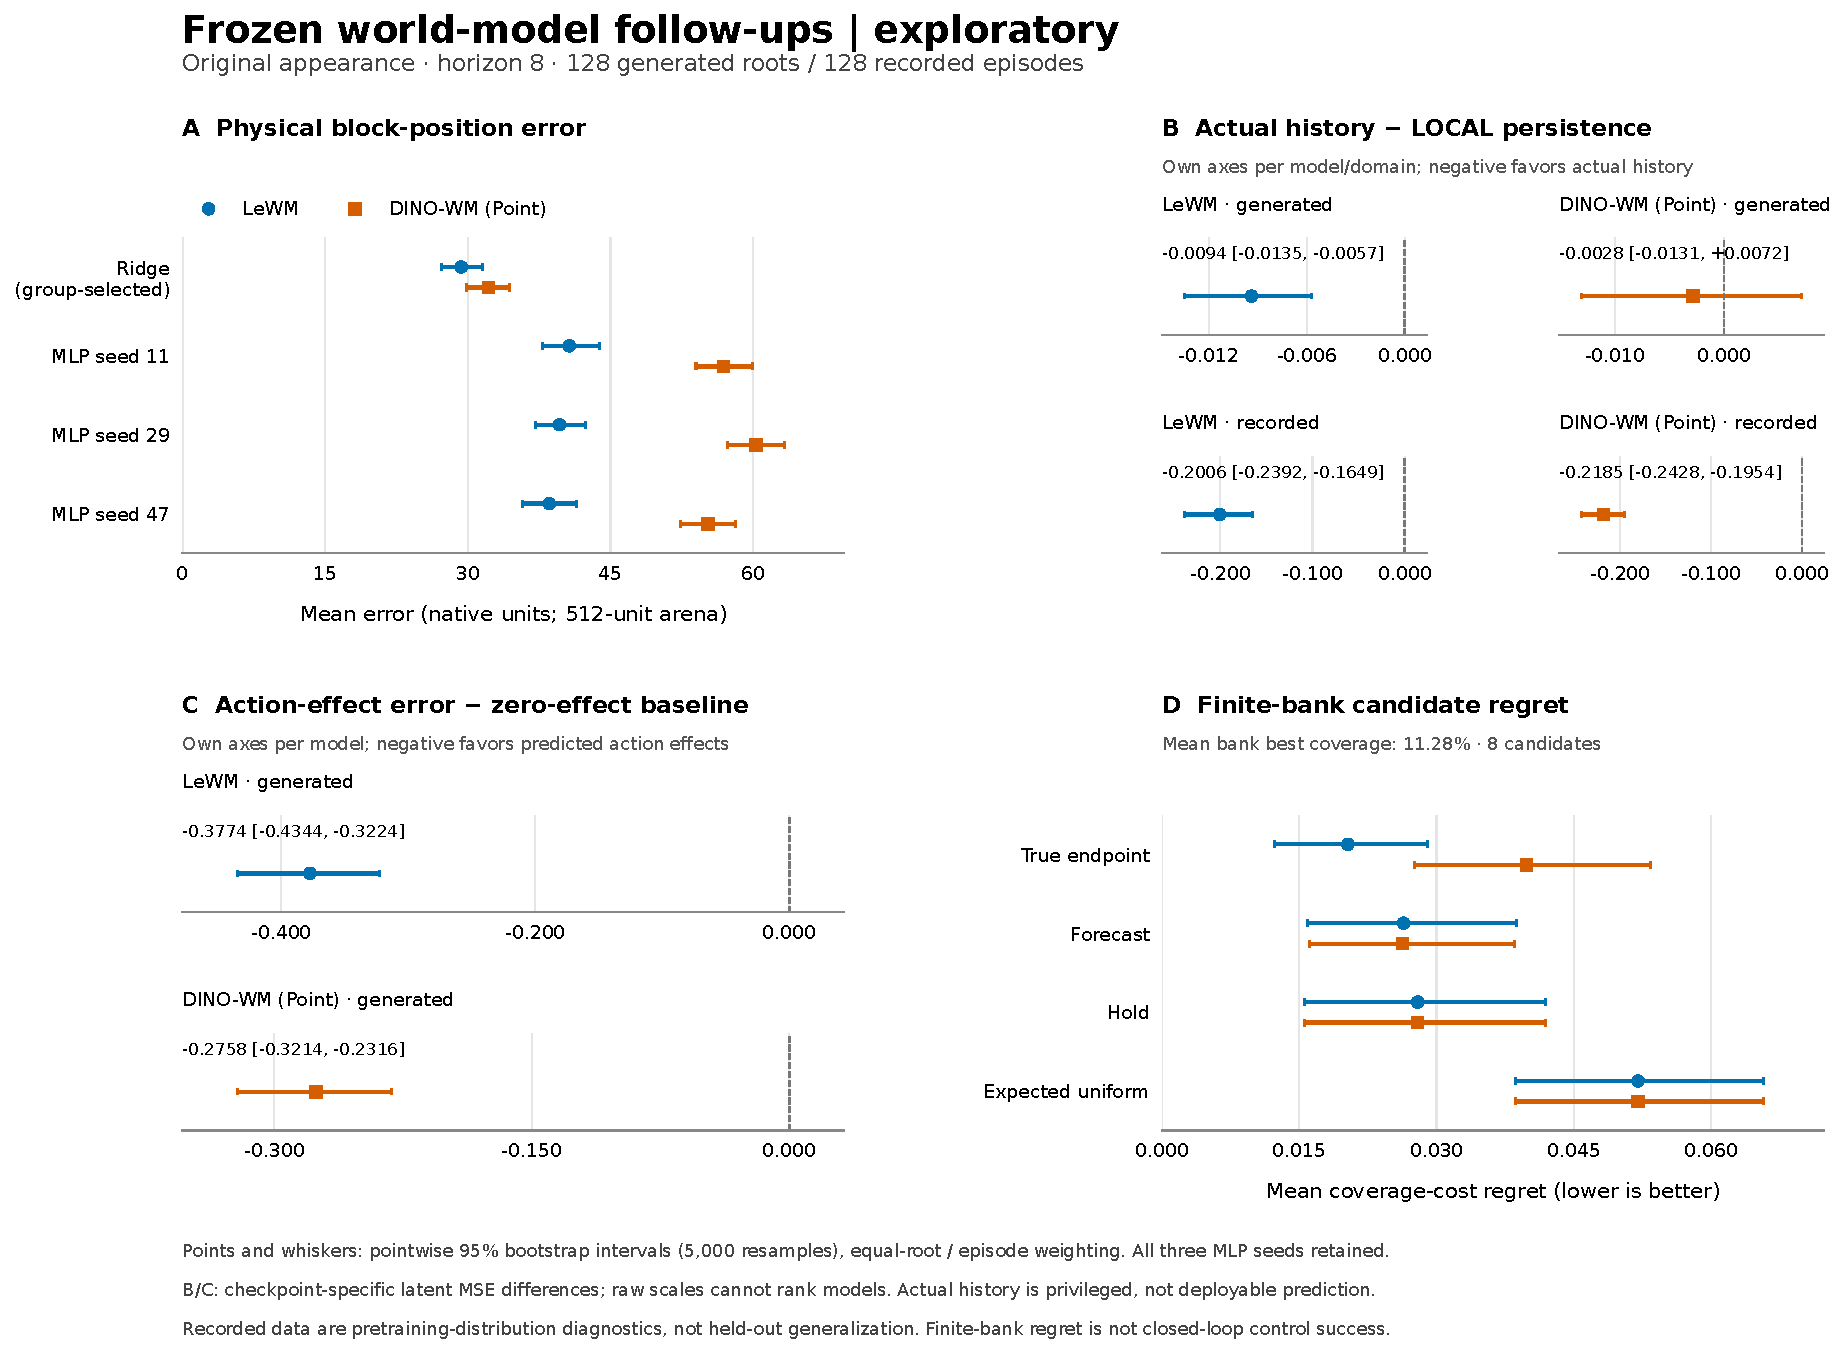
\includegraphics[width=.98\textwidth]{generated/discovery_summary.pdf}
\caption{Authenticated discovery follow-up summary. All probe seeds, oracle/
local-persistence controls, action contrasts and finite-bank regrets are
exploratory pointwise 95\% views on inspected data. These intervals must not be
read as the independent primary-family results in Figure \ref{fig:primary}.}
\label{fig:discovery}
\end{figure}

\section{Primary and Complementary Inference}
\label{app:inference}

The original manifest includes all five split names, including an empty
confirmation roster. Every original archive is authenticated before fresh-root
generation. Fresh root IDs, 128-bit root seeds and environment seeds are checked
against old and reserved identities. The generator retains the native bank,
clearance 2 and maximum 256 initial-anchor attempts; no bank improvement,
contact/visibility screening or outcome filtering is inserted.

Root means are ordered by full root ID. The saved $10000\times128$ int64
bootstrap matrix is generated once by NumPy PCG64 with seed 20261102 and used
for both models and all contrasts. Primary quantiles are 0.005/0.995, linear
interpolation. The five-member family includes Equations \ref{eq:fidelity}
and \ref{eq:specificity} for each model and forecast-minus-endpoint regret for
DINO only. Every primary estimate and interval is reported even if another
member is inconclusive. All-primary replication requires all five; that
criterion was not met.

The effect gain is $g=\overline{\langle\Delta P,\Delta A\rangle}/
\overline{\lVert\Delta A\rVert^2}$, using equal-root means after candidate
and branch averaging. If any resampled denominator is zero, the unconditional
interval is undefined and the count is reported rather than conditioning on
nonzero draws. Both fresh gains have zero undefined draws. An energy ratio
near one and $g<1$ are compatible with misaligned/off-axis effects; a
pure insufficient-amplitude explanation is not established.

The untouched underlying dynamics reports retain their legacy exploratory
schema and inspected-pilot boilerplate. Fresh sample identity and primary
inference are established by the new plan, composite data manifest and joint
analysis, not by rewriting legacy report tags. All 1,680 exploratory
estimates/intervals and five primary contrasts were independently recomputed;
maximum comparison discrepancy was $2.27\times10^{-13}$. The numerical verifier
checks 1,800 summary statistics per model with rounding discrepancy at most
$1.11\times10^{-16}$.

\begin{figure}[h]
\centering
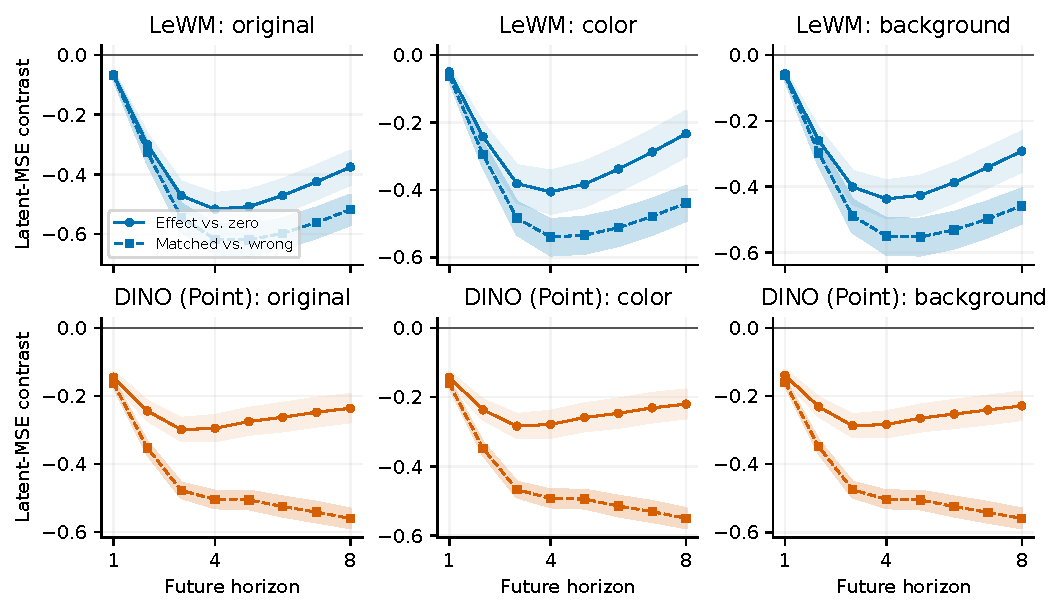
\includegraphics[width=.97\textwidth]{generated/replication_slices.pdf}
\caption{All fresh-sample horizons and appearances for the two action
contrasts. Shaded intervals are pointwise exploratory 95\%, including the
primary metrics' exploratory views. Only original appearance/horizon 8 uses
the dedicated 99\% primary family. No favorable slice is selected to replace
the inconclusive decision result. Raw latent scales remain model-specific.}
\label{fig:slices}
\end{figure}

\begin{table}[h]
\caption{Complementary fresh-sample summaries at every appearance and the
original reporting horizons. Every interval is pointwise exploratory 95\%.
Fidelity and feedback use model-specific latent MSE; forecast--hold uses native
coverage-cost regret. No row is an additional primary claim.}
\centering\small
% Generated from authenticated reports; do not edit.
\begin{tabular}{lllrrr}
\toprule
Model & Appearance & $h$ & Oracle--local persistence & Effect--zero & Forecast--hold \\
\midrule
LeWM & original & 1 & -0.0529 [-0.0633, -0.0435] & -0.0645 [-0.0762, -0.0539] & -0.0008 [-0.0038, 0.0022] \\
LeWM & original & 4 & -0.0572 [-0.0693, -0.0463] & -0.5162 [-0.5715, -0.4639] & 0.0063 [-0.0001, 0.0133] \\
LeWM & original & 8 & -0.0112 [-0.0148, -0.0078] & -0.3753 [-0.4329, -0.3221] & 0.0034 [-0.0047, 0.0116] \\
LeWM & color & 1 & -0.0389 [-0.0501, -0.0285] & -0.0493 [-0.0618, -0.0377] & -0.0010 [-0.0038, 0.0018] \\
LeWM & color & 4 & -0.0430 [-0.0559, -0.0312] & -0.4057 [-0.4695, -0.3441] & 0.0073 [-0.0012, 0.0164] \\
LeWM & color & 8 & 0.0038 [-0.0018, 0.0098] & -0.2333 [-0.2996, -0.1671] & 0.0051 [-0.0019, 0.0123] \\
LeWM & background & 1 & -0.0459 [-0.0568, -0.0363] & -0.0566 [-0.0689, -0.0457] & -0.0002 [-0.0033, 0.0028] \\
LeWM & background & 4 & -0.0532 [-0.0654, -0.0420] & -0.4374 [-0.4943, -0.3825] & 0.0076 [-0.0006, 0.0163] \\
LeWM & background & 8 & -0.0069 [-0.0109, -0.0032] & -0.2920 [-0.3531, -0.2334] & 0.0085 [0.0001, 0.0178] \\
DINO (Point) & original & 1 & -0.0625 [-0.0784, -0.0459] & -0.1450 [-0.1592, -0.1301] & -0.0016 [-0.0042, 0.0004] \\
DINO (Point) & original & 4 & -0.0015 [-0.0151, 0.0116] & -0.2953 [-0.3319, -0.2578] & -0.0079 [-0.0154, -0.0018] \\
DINO (Point) & original & 8 & 0.0029 [-0.0070, 0.0130] & -0.2364 [-0.2763, -0.1961] & -0.0033 [-0.0127, 0.0046] \\
DINO (Point) & color & 1 & -0.0575 [-0.0738, -0.0406] & -0.1425 [-0.1567, -0.1276] & -0.0007 [-0.0032, 0.0014] \\
DINO (Point) & color & 4 & 0.0049 [-0.0081, 0.0175] & -0.2787 [-0.3158, -0.2409] & -0.0080 [-0.0155, -0.0020] \\
DINO (Point) & color & 8 & 0.0036 [-0.0060, 0.0135] & -0.2202 [-0.2603, -0.1793] & -0.0040 [-0.0134, 0.0040] \\
DINO (Point) & background & 1 & -0.0317 [-0.0479, -0.0148] & -0.1389 [-0.1527, -0.1245] & -0.0012 [-0.0033, 0.0005] \\
DINO (Point) & background & 4 & 0.0323 [0.0186, 0.0459] & -0.2837 [-0.3200, -0.2467] & -0.0068 [-0.0140, -0.0011] \\
DINO (Point) & background & 8 & 0.0330 [0.0226, 0.0436] & -0.2289 [-0.2691, -0.1886] & -0.0054 [-0.0155, 0.0030] \\
\bottomrule
\end{tabular}

\end{table}

\section{Numerical Audit Matrix and Limits}
\label{app:numerics}

The eight-root numerical audit retains both branches, all candidates and
common actual horizons 1/4/8. The old path encodes context as batches 4,2,
encodes each candidate's three selected future frames together, and invokes
public single-candidate native and zero-action rollouts. The new path retains
context/goal/future encoding calls, the actual free/oracle control suite and
its public eight-candidate parity call. Controlled bridges cross old/new
encoded context and targets with single/bank public rollouts. The bank layout
includes observed strides; it does not isolate GEMM batch size alone.

Each observed suite executes twice with unchanged incoming backend settings.
Four distinct controls are then applied individually: matmul IEEE, matmul TF32,
convolution IEEE and cuDNN deterministic. Benchmark-off is already off. Every
property is restored in a finally block, including precision inheritance;
unavailable legacy getters under modern overrides are recorded explicitly.
This yields seven within-setting comparisons for baseline and each control,
five repeat comparisons and five baseline/control variant comparisons per
control: 60 groups with 128 matched records each. The controls were specified
before inspecting their outcomes.

Native float32 and common CPU float64 metric reductions are stored. Tensor
maximum/mean absolute differences have full root/branch/candidate/horizon
identities. Same-layout repeats, matmul IEEE and cuDNN deterministic produce
no observed changes on this sample. Other settings shift the encoded targets
as well as predictions. Permissions do not prove which backend kernel was
selected. CUDA/cuDNN cache history, driver, attention backend, allocator and
concurrent workloads are not reset or exhaustively varied. Historical
backend state and full raw tensors were not saved, so historical causal
attribution and cross-process portability remain unresolved.

\section{Reporting and Extension Boundaries}
\label{app:extension}

This paper is an evidence checkpoint, not a commitment to obtain a positive
result by further search. Future observability-aware history probes,
state-specific action-effect readouts and contact/reachable-bank or closed-loop
decisions would need separate hypotheses, competing alternatives, frozen
selection, fresh evaluation and failure-preserving protocols. They cannot be
inserted as results until actually run and verified. A qualified editor study
depends first on physical-change measurement at adequate resolution. Any
new bank changes the task distribution and must be labeled accordingly.

No claims of priority for diagnostic separation or a new world-model method
are made. Close grounding, intervention and decision-alignment papers are
cited in Section \ref{sec:related}. Final bibliographic versions, venue rules,
anonymity, author contributions, disclosure and redistribution terms require
author review. ICML style is a typesetting choice for this draft, not evidence
of submission, acceptance or compliance with a future call.